\documentclass[a4paper]{scrartcl}
\usepackage[utf8]{inputenc}
\usepackage[english]{babel}
\usepackage{graphicx}
\usepackage{lastpage}
\usepackage{pgf}
\usepackage{wrapfig}
\usepackage{fancyvrb}
\usepackage{fancyhdr}
\usepackage{float}
\usepackage{xurl}
\usepackage{hyperref}
\pagestyle{fancy}

% Create header and footer
\headheight 27pt
\pagestyle{fancyplain}
\lhead{\footnotesize{Data Storage Paradigms, IV1351}}
\chead{\footnotesize{Project Report}}
\rhead{}
\lfoot{}
\cfoot{\thepage\ (\pageref{LastPage})}
\rfoot{}

\title{Project Report Task 3}
\subtitle{Data Storage Paradigms, IV1351}
\author{}
\date{2024-12-02}

\begin{document}

\maketitle
\noindent\textbf{Project members:} \\ \hfill
Jonathan Värild, varild@kth.se \\ \hfill
Oscar Caddeo, ocaddeo@kth.se \\ \hfill
Elias Holm, eliholm@kth.se \\ \hfill

\section*{Declaration:}

By submitting this assignment, it is hereby declared that all group members listed above have contributed to the solution. It is also declared that all project members fully understand all parts of the final solution and can explain it upon request.

It is furthermore declared that the solution below is a contribution by the project members only, and specifically that no part of the solution has been copied from any other source (except for lecture slides at the course IV1351), no part of the solution has been provided by someone not listed as a project member above, and no part of the solution has been generated by a system.

\section{Introduction}


\section{Literature Study}
Our primary source of information for this assignment was the PostgreSQL documentation available at \url{https://www.postgresql.org/docs/current/}. This provided valuable information and even examples on how to write different queries. The chapters 6 and 7 in the book also provided valuable information on how to structure the actual queries and how to work with the data. For example, \textbf{7.1 More Complex SQL Retrieval Queries} mentions uses of the different functions such as \textbf{SUM}, how to work with \textbf{GROUP BY}, joining tables, etc. They also provide very good examples with images and diagrams which further help to visualize the concepts.

\section{Method}


\section{Result}

The GitHub repository with Astah files, SQL files, etc., can be found at \url{https://github.com/Cadde0/IV1351-Project}.

\subsection{Query 1: Show the number of lessons given per month during a specified year}
See code: \url{https://github.com/Cadde0/IV1351-Project/blob/da393a327bdfa9095d946e80d1bcf94df4ccb866/queries.sql#L1}.

The first query we created was for retrieving information about how many activities there are of each type, each month.

The query works using a \textbf{SELECT} operation on the \textbf{activity} table which is \textbf{LEFT JOIN}:ed with \textbf{lesson\_individual}, \textbf{lesson\_group}, and \textbf{ensamble} where their \textbf{activity\_id} matches. Basically, what we do is that we take all the activities and get the full information of each activity from the respective table depending on the activity type. \textbf{LEFT JOIN} allow us to join the \textbf{activity} table with all the tables at once (\textbf{lesson\_individual}, \textbf{lesson\_group}, and \textbf{ensamble}), but each join will only affect matching rows for each activity. If we were to use normal \textbf{JOIN}, we would lose a lot of rows where matches weren't found since each activity only is linked with 1 of the 3 activity tables.

The data is filtered using a \textbf{WHERE} clause where we extract the year from the \textbf{start\_time} column of each activity, and compare it to a number representing the year we want to look at. This ensures only activities from that year are included, as per the assignment requirements. If you want to look at other years, you need to modify the number value for that comparison.

The \textbf{GROUP BY} clause ensures that all the activities are grouped by their month. The reason why we group the rows by both the text based month and the numerical month is since we use the numerical month for sorting, and therefore have to include it. 

Finally, the \textbf{ORDER BY} clause where we sort the rows based on the numerical value of each month.

\begin{figure}[H]
    \begin{center}
      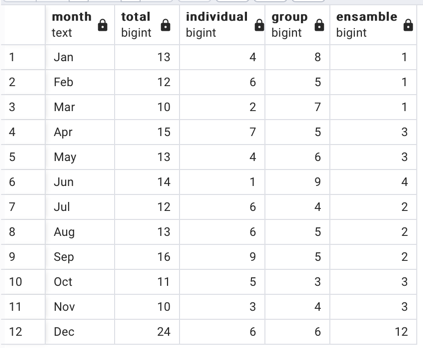
\includegraphics[scale=0.6]{query1_output.png}
      \caption{The output from performing query 1 on our database with the test data provided in the GitHub repository.}
      \label{fig:diag}
    \end{center}
  \end{figure}


\subsection{Query 2: Show how many students there are with no sibling, with one sibling, with two siblings, etc.}
See code: \url{https://github.com/Cadde0/IV1351-Project/blob/da393a327bdfa9095d946e80d1bcf94df4ccb866/queries.sql#L25}.

The second query will list how many students that different number of siblings registered in the school database.

First, we want to get all sibling relations that there is in our database. All siblings are registered in a table called \textbf{sibling} which consists of two columns corresponding to two student school IDs that link the two students together. To ensure that there are no duplicate rows for two students, the two rows are a composite primary key and a trigger enforces that the two student school IDs are ordered with the smallest school ID in the first column and the largest in the second column.

Therefore, we make two \textbf{SELECT} operations. First we make one where we select all \textbf{student\_school\_id\_first} and count the number of \textbf{student\_school\_id\_second}. Since we count the number of \textbf{student\_school\_id\_second}, we of course have to use \textbf{GROUP BY} on \textbf{student\_school\_id\_first}. After that we do exactly the same \textbf{SELECT} operation, but we swap \textbf{student\_school\_id\_first} and \textbf{student\_school\_id\_second}. To merge these operations, we use \textbf{UNION ALL} between them. These operations are done in a Common Table Expression (CTE) called \textbf{sibling\_count} to increase readability. Next, we have another CTE called \textbf{total\_sibling\_count} where we sum up the number of siblings that we counted respectively for each column in the previous CTE.

Finally, we display the information using a \textbf{SELECT} operation. Since we also want to know how many students that there are without siblings, we make the \textbf{SELECT} operation on the \textbf{student} table. We \textbf{LEFT JOIN} all students with our CTE \textbf{total\_sibling\_count} on their student IDs which ensures that we only join students that have siblings, but still keep the rows of student that doesn't have siblings. We select the \textbf{no\_of\_siblings\_sum} from each student as \textbf{"No of Siblings"} and use the function \textbf{COALESCE} to ensure that \textbf{NULL} values are replaced by \textbf{0}, since this are students without siblings that weren't matched up with our \textbf{LEFT JOIN} clause. Next, we select \textbf{COUNT} with all rows as \textbf{"No of Students"} to count the number of students for each number of siblings.

Finally, we use a \textbf{GROUP BY} clause to group everything by the number of siblings. We also use a \textbf{ORDER BY} clause to order the rows by the number of siblings. The result can be seen in Figure 2 below.

\begin{figure}[H]
    \begin{center}
      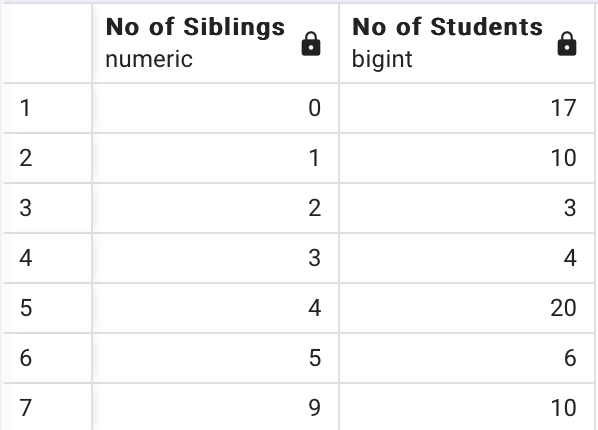
\includegraphics[scale=0.6]{query2_output.png}
      \caption{The output from performing query 2 on our database with the test data provided in the GitHub repository.}
      \label{fig:diag}
    \end{center}
  \end{figure}


\subsection{Query 3: List ids and names of all instructors who has given more than a specific number of lessons during the current month.}
See code: \url{https://github.com/Cadde0/IV1351-Project/blob/da393a327bdfa9095d946e80d1bcf94df4ccb866/queries.sql#L61}.

In this query we will select the instructor ID, first name, last name, and the number of lessons that each instructor has given during the current month. In our example, we limited the number of lessons to \textbf{0} to show more data, but this number can obviously easily be changed to only show instructors that has given a certain number of lessons.

The query starts with a CTE called \textbf{lessons\_this\_month} which contains a \textbf{SELECT} operation on the \textbf{activity} table. We select the \textbf{instructor\_school\_id} column and use \textbf{COUNT} as \textbf{total\_lessons} on all rows to count the number of lessons that each instructor is assigned on. Since we use \textbf{COUNT} we also have to use a \textbf{GROUP BY} clause on the \textbf{instructor\_school\_id} column. To enforce that we only count lessons that were given during the last month we have a \textbf{WHERE} clause where we check that the month and year of the \textbf{start\_time} column on each activity is the same as our current month and year.

Now we only have the instructor ID and the number of lessons that each instructor ID has given. To connect this information with a real person, we finally make a new \textbf{SELECT} operation on \textbf{lessons\_this\_month} and join this data with the \textbf{person} table on the instructor ID. This allows us to finally select the first and last name of the instructor. It's here that we have a \textbf{WHERE} clause where we can decide the lower limit of lessons to include the instructor. Finally, we have a \textbf{ORDER BY} clause that orders everything by \textbf{"No of Lessons"}.

\begin{figure}[H]
    \begin{center}
      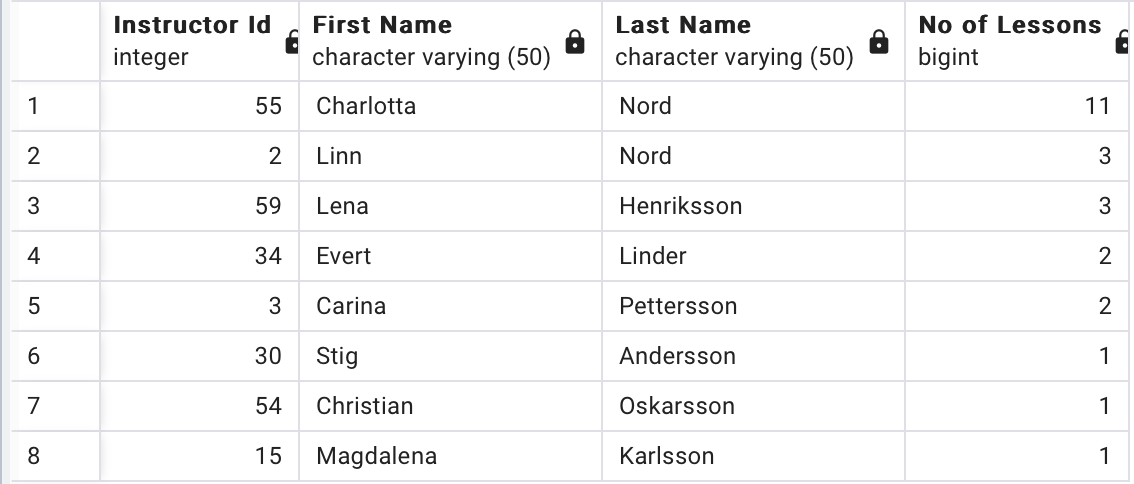
\includegraphics[scale=0.6]{query3_output.png}
      \caption{The output from performing query 3 on our database with the test data provided in the GitHub repository.}
      \label{fig:diag}
    \end{center}
  \end{figure}

\subsection{Query 4: List all ensembles held during the next week}
See code: \url{https://github.com/Cadde0/IV1351-Project/blob/da393a327bdfa9095d946e80d1bcf94df4ccb866/queries.sql#L84}.

This query will give us a schedule-like output of all ensembles next week and also include the number of free seats for each ensemble.

We start by defining a CTE called \textbf{ensambles\_next\_week} where we have a \textbf{SELECT} operation from activity. This table is in turned \textbf{JOIN}:ed with the \textbf{ensamble} table where their activity IDs match to only include activities that are ensembles. This also gives us access to all the information about each ensemble. We use a \textbf{WHERE} clause where we check so the \textbf{start\_time} of the ensemble is within the first and last day of next week.

Next, we create another CTE called \textbf{bookings\_per\_ensamble} where we count the number of bookings for each ensemble. We do this using a \textbf{SELECT} operation on \textbf{ensambles\_next\_week} which is joined using \textbf{LEFT JOIN} on the \textbf{booking} table where their activity ID matches. We select the activity ID and use \textbf{COUNT} to count the number of rows for this activity.

Finally, we make an \textbf{SELECT} operation on \textbf{ensambles\_next\_week} and \textbf{LEFT JOIN} this with \textbf{bookings\_per\_ensamble} where their activity IDs match. We select the weekday using the \textbf{TO\_CHAR} function with the \textbf{start\_time} column, genre, and use a \textbf{CASE} clause to show different texts for the \textbf{"No of Free Seats" } column based on the number of seats left. We use the \textbf{COALESCE} function to ensure that we have a \textbf{0} to compare with for \textbf{NULL} values where there are no bookings. Finally, we use a \textbf{ORDER BY} clause to order everything first by \textbf{Day} and then by \textbf{Genre}.



\begin{figure}[H]
    \begin{center}
      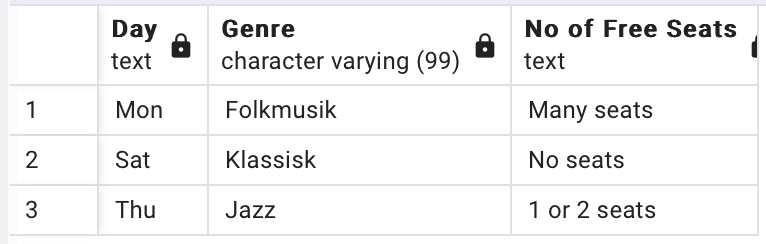
\includegraphics[scale=0.6]{query4_output.png}
      \caption{The output from performing query 4 on our database with the test data provided in the GitHub repository.}
      \label{fig:diag}
    \end{center}
  \end{figure}


\subsection{Query 5: Query for selecting and inserting historical data in denormalized database}
See code: \url{https://github.com/Cadde0/IV1351-Project/blob/da393a327bdfa9095d946e80d1bcf94df4ccb866/queries.sql#L116} and \url{https://github.com/Cadde0/IV1351-Project/blob/main/CreateHistorical.sql}.

This last query is part of the higher grade task, where we are assigned to select all activities that people have made bookings for into a denormalized database. We have also created the historical database diagram which can be seen in \textbf{Figure 5} below. To make it easier to move the data to the \textbf{activity\_history} table with a single query we implemented it into the same database. This might be bad practice because you don't necessarily want to fill up your main production database with historical data that is based on data within it. Instead, it would be a great idea to offload this data to a database that only keeps historical data. However, moving data between databases like this isn't introduced in this course.

The \textbf{activity\_history} table consists of a composite primary key of \textbf{student\_school\_id} and \textbf{activity\_id} which ensures that there can only be one row for each activity and student. This effectively eliminates the possibility of duplicate rows for the same booking. Next, we have the \textbf{activity\_type} column which is implemented as a enum defined in the connected note. Next, we have the \textbf{activity\_price} which is the final price for the activity, based on the hourly price of the activity and its length. The \textbf{activity\_price} also have a check to ensure that it isn't negative, since this would be unlogical. After that we have the \textbf{instrument} and \textbf{genre} columns which are allowed to be \textbf{NULL}, but uses checks to ensure that they only are \textbf{NULL} when allowed depending on the \textbf{activity\_type}. Lastly, we have the student's first name, last name, email and the date of the activity. You could denormalize the database even more by combining the first and last name into a single column, but we chose to separate them because we believe that there might be practical reasons to still be able to easily differentiate this later if you need to use this historical data.

Looking back at the query, we start with a CTE called \textbf{personal\_emails} where we have a \textbf{SELECT} operation which selects \textbf{DISTINCT} \textbf{school\_id}, \textbf{email} and a \textbf{school\_id}. We have a \textbf{WHERE} clause which ensures that we only select rows that have personal contact details and an email address. Basically, what we do is that we select all personal email addresses registered, but only one per \textbf{school\_id} since our denormalized database only allows one email, per booking.

Next, we have a CTE called \textbf{history\_data} which basically joins and merges all data that we need to later make the \textbf{INSERT} operation into the denormalized \textbf{activity\_history} table. It starts with a \textbf{SELECT} operation on the \textbf{booking} table, since it is the bookings we are interested in. We join this table with \textbf{person} to get access to the person name, etc., behind each booking. We use \textbf{LEFT JOIN} on \textbf{personal\_emails} to join the email addresses of all students that have a personal email registered. The \textbf{activity} table is joined to get access to activity data such as the start time, end time, and activity type. The \textbf{pricing} table is joined, so we can retrieve pricing data that can be calculated using the start and end time in the \textbf{activity} table. We use \textbf{LEFT JOIN} on \textbf{lesson\_individual}, \textbf{lesson\_group}, and \textbf{ensamble} to join the bookings only with its matching activity. Finally, we make a join with \textbf{instrument\_type} to get the name of the instrument for all the lessons.

All this data is selected pretty easily except from \textbf{activity\_length\_hours} that is calculated from the start and end time of the activity, and \textbf{activity\_type} that is made into an \textbf{activity\_type\_enum} as needed by the \textbf{activity\_history} table,

A final \textbf{INSERT} operation then uses a \textbf{SELECT} operation to get the data from \textbf{history\_data} and insert it into \textbf{activity\_history}. The \textbf{activity\_price} is calculated by multiplying the columns \textbf{activity\_length\_hours} and \textbf{hourly\_price}.

Running the query multiple times will not be a problem due to the final clause \textbf{ON CONFLICT} which ignore rows that already have been inserted. However, you would probably also want to include a \textbf{WHERE} clause that ignores activities before a certain date. Nothing about this is however mentioned in the assignment, so this is just something we considered ourselves. The query will run just fine for moving data without \textbf{ON CONFLICT} as long as you don't run it on the same data set twice.

\begin{figure}[H]
    \begin{center}
      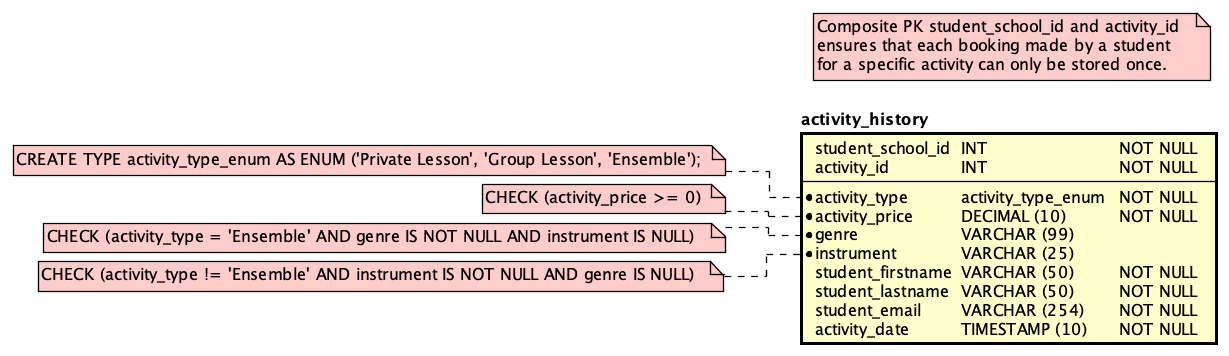
\includegraphics[scale=0.4]{Denormalized Historical Database.png}
      \caption{Diagram of our denormalized database for storing historical data.}
      \label{fig:diag}
    \end{center}
  \end{figure}

\section{Discussion}

\subsection{Question 1}

\subsection{Question 2}

\subsection{Question 3}

\subsection{Advantages and disadvantages of using denormalization}
Denormalized databases are often used in implementations where you want to favor read speeds. Its main advantages include better performance for reading data due to fewer uses of joins and potentially better indexing. It also makes queries a lot easier to understand since you won't have to work with a lot of tables like you do in a normalized database.

One of the obvious disadvantages is bigger database size since you store a lot of the same data multiple times. It might also be hard to maintain a denormalized database if you need to modify the same data at multiple locations. This can become time-consuming for its maintainers and makes it prone to errors. It will also be a lot more performance heavy if you for example need to update the same data at multiple locations. If you are working with huge amounts of data, you also pose the risk of meeting the limitations of your database quicker. This might for example arise as performance degradation, etc.

\section{Comments About the Course}

\end{document}
